\section{Precursor: Method of Lagrange Multipliers}


\begin{frame}\frametitle{\secname} 
    \begin{center}
    \slidesonly{\huge}
	Don't panic!
    \end{center}
    \begin{center}
        Essentially just hill-climbing (gradient ascent)
    \end{center}
    \pause

\underline{Objective}: \\
\textit{Maximize} an objective function while also satisfying some constraint(s).\\
{
\small(\textit{Maximize}: Find the arguments that maximize an objective function.)
}\\[5mm]
Don't forget: any maximization problem can be turned into a minimization problem\notesonly{ by maximizing the ``negative'' of the function}.
\end{frame}

\subsection{Gradient ascent - unconstrained optimization}
\begin{frame}\frametitle{\subsecname}
Maximize an objective function $f(w_1, w_2)$ (no constraints here).\\
Here $w_1$ and $w_2$ are referred to as free parameters.\\

\begin{figure}[h]
	\centering
	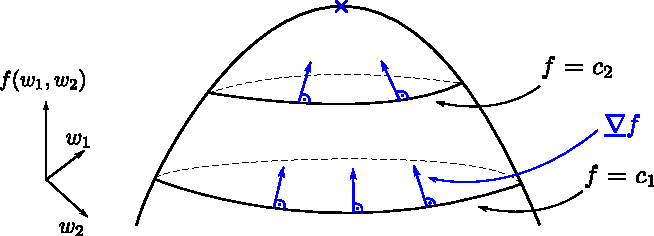
\includegraphics[width=0.8\linewidth]{img/lagrange_objfunction.pdf}
	\mode<article>{
	\caption{
	The objective function $f$ we want to maximize (i.e. reach the blue ${\color{blue}\times}$ at the top). $c_1$ and $c_2$ are level curves where $f$ is constant. 
	The blue arrows indicate the direction of the gradient $\vec \nabla f$, which is always perpendicular to the level curve.
	}
	}
\end{figure}
\slidesonly{
\vspace{-3mm}
}
The gradient $\vec \nabla f$ describes the direction of greatest ascent:\\
\slidesonly{
\vspace{-3mm}
}
\begin{equation}
\vec \nabla f = 
\frac{\partial f}{\partial \vec w} = 
\rmat{\frac{\partial f}{\partial w_1} \\[0.2cm] \frac{\partial f}{\partial w_1} }
\end{equation}

\end{frame}


\newpage

\subsection{Adding a constraint}
\begin{frame}\frametitle{\subsecname}
We restrict solutions to those that satisfy the constraint $g(w_1, w_2) = c$:

\begin{figure}[h]
\centering
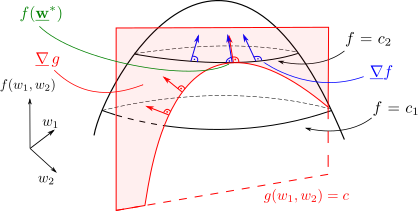
\includegraphics[width=0.7\linewidth]{img/lagrange_objfunction_constrained}
\mode<article>{
\caption{The surface of the constaint cuts through the surface of the objective function. The highest point that can be reached on $f$ which also intersects with $g$ is unique in that the gradients of $f$ and $g$ both point in the same direction with only a difference in scale.}
}
\end{figure}

\question{What is characteristic of the solution to the constrained optimization problem?}

\notesonly{
-The solution of the constrained optimization problem is characterized by:
}
\begin{equation}
    \vec \nabla f = \lambda' \vec \nabla g\,,\quad
\text{where $\lambda'$ is a scaling factor.}
\label{eq:equality}
\end{equation}

\notesonly{\eqref{eq:equality} holds for the highest position in $f$ while also satisfying the constraint.}
Consequently,

\begin{align}
  \vec \nabla f \; - \lambda' \vec \nabla g     &= \vec 0 \\
  \vec \nabla f \; + \underbrace{(- \lambda')}_{=:\lambda} \vec \nabla g &= \vec 0 \\
  \vec \nabla f \;  + \lambda \vec \nabla g      &= \vec 0 \text{ (to be more consistent with lecture slides.})
\end{align}

\end{frame}

\begin{frame}
%\newpage
The optimization problem is thus:

\begin{equation}
\underbrace{f(w_1, w_2) \;\eqexcl\; \max_{w_{1},w_{2}}}_{\text{maximization}} \quad  \text{subject to} \quad \underbrace{g(w_1,w_2)\;-c\; = \; 0}_{\text{one constraint}}
\end{equation}

\newpage
The Lagrangian function is then defined as:

$$
L(w_1, w_2, \lambda) \; = \; f(w_1,w_2) + \lambda(g(w_1, w_2)-c)
$$

Setting the gradient $\nabla L$ to zero guarantees $\vec \nabla f \;  + \lambda \vec \nabla g = \vec 0$

$$
\vec \nabla L = 
\rmat{
	\frac{\partial L}{\partial w_1} \\[0.3cm]
	\frac{\partial L}{\partial w_2} \\[0.3cm]
	\frac{\partial L}{\partial \lambda}
	}
=
\rmat{
	\frac{\partial f}{\partial w_1} \quad+\quad \lambda \frac{\partial g}{\partial w_1} \\[0.3cm]
	\frac{\partial f}{\partial w_2} \quad+\quad \lambda \frac{\partial g}{\partial w_2} \\[0.3cm]
	\underbrace{\frac{\partial f}{\partial \lambda}}_{=0} \;+\; g(w_1, w_2)-c
	}
$$

Setting the first two elements in $\nabla L$, namely $\frac{\partial L}{\partial w_1}$ and $\frac{\partial L}{\partial w_2}$, to zero ensures that $\nabla f = -\lambda \nabla g$,\\
while $\frac{\partial L}{\partial \lambda}=0$ ensures that $g(w_1, w_2) = c$.\\

3 equations, 3 unknowns.\\

We refer to $\lambda$ as the multiplier for constraint $c$.


\subsection{How do we extend this to multiple constraints?}

$$
\underbrace{f_0(\vec w) \;\eqexcl\; \text{max}}_{\text{maximization}} \quad  \text{and} \quad f_k(\vec w)\;\le\; = \; 0 \;, \quad k = 1,\ldots,m
$$

where $m$ denotes the number of constraints.

The Lagrangian is then defined as:

$$
L(\,\vec w\;, \underbrace{\{\lambda_k\}}_{
\mathclap{
\substack{\text{a multiplier} \\
\text{for each constraint}}
}
}) \; = \; f_0(\vec w) + \sum_{k=1}^{m} \lambda_k \, f_k(\vec w)
$$


\end{frame}

